\documentclass[10pt,a4paper,oneside]{article}
\usepackage{amsmath,amsthm,amssymb,floatrow}
\usepackage{lmodern}
\usepackage{geometry}
\usepackage{graphicx,float,subfigure,ctex}
\DeclareGraphicsExtensions{.pdf,.jpeg,.png,.jpg}
\geometry{left=2.18cm,right=2.18cm,top=1.54cm,bottom=2.0cm}
\pagestyle{empty}
\title{\bf 运筹学实验报告-2}
\author{姓名:李奕萱  学号:PB22000161 }
\date{\today}

\begin{document}

\maketitle

\section{问题背景}

在图论中,最短路径问题是最基本也是最重要的问题之一,
广泛应用于通信网络、交通调度、地图导航等领域。对于给
定的加权图,最短路径问题旨在寻找从源点到目标点的路径
,使得路径上的总权重最小。为了求解最短路径问题,许多
算法被提出,其中最常用的算法包括Dijkstra算法和线性
规划(LP)方法。Dijkstra算法能够在加权图中高效地求
解单源最短路径问题,但在某些情况下,尤其是在图的规
模较大时,运行时间可能变得较长。与此相对,LP方法通
过建立优化模型来求解最短路径问题,尽管它的计算时间
在大规模问题中可能会较长,但可以处理更复杂的约束条件。

本实验通过对比Dijkstra算法与LP方法在求解最短路径问题
中的表现,探索不同规模图的求解效率,并通过实验结果分析
它们的优缺点。

\section{算法介绍}

\subsection{随机产生图}

\begin{figure}[H]
    \centering
    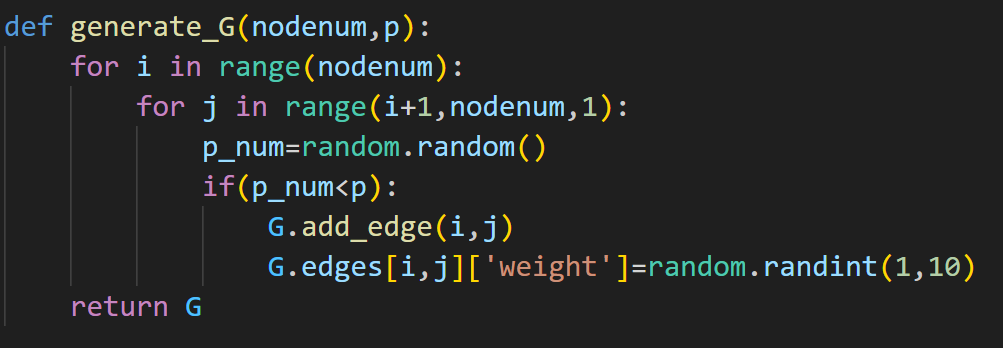
\includegraphics[width=0.8\textwidth]{屏幕截图 2024-10-18 132429.png}
\end{figure}

本实验中,使用$networkx\ package$ 生成$ER(n,p)$图,
图中共$n$个点,每条边以概率$p$连接。

- 若$p<\frac{(1-\epsilon)\ln n}{n}$,则图中几乎必有一个孤立点。
此时会自动删除孤立点,$n$减少。

- 若$p>\frac{(1+\epsilon)\ln n}{n}$,则图几乎必然连通。

为了确保图的连通性,本实验中选择$p=0.8$,并为每条生成
的边随机赋予一个距离,取值范围为$1-10$的整数。

\subsection{dijksta算法实现}

\begin{figure}[H]
    \centering
    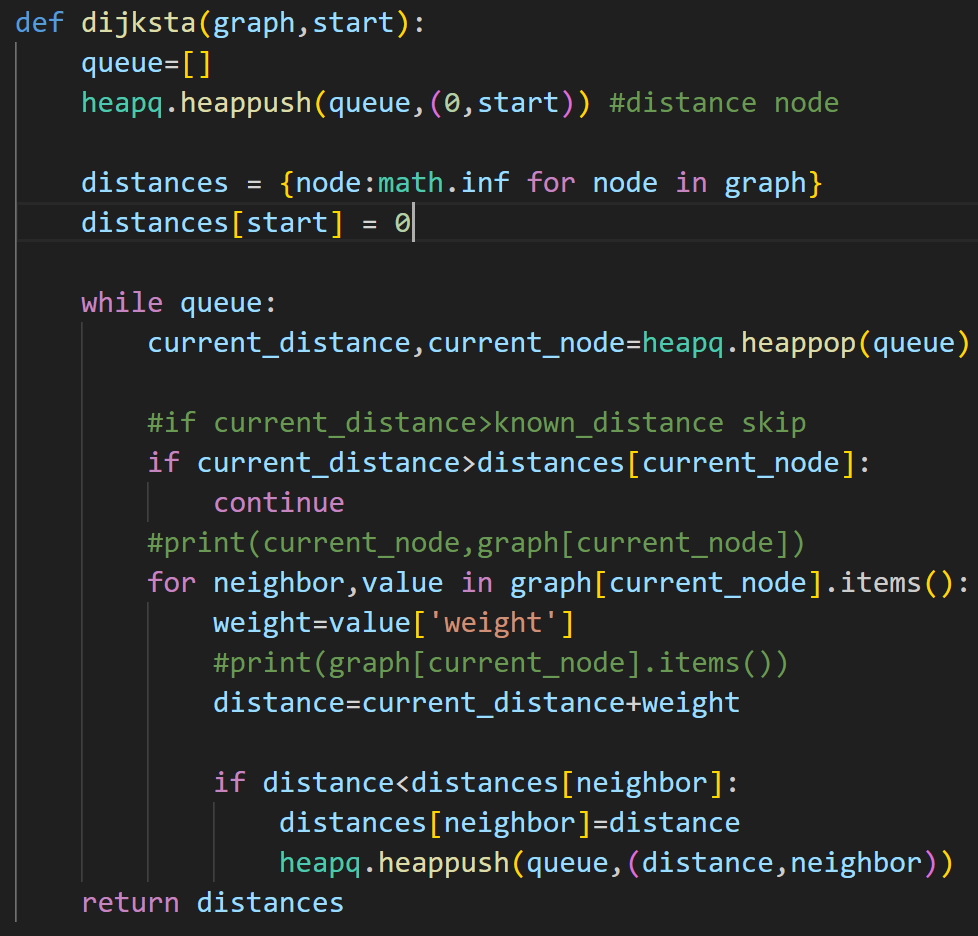
\includegraphics[width=0.8\textwidth]{屏幕截图 2024-10-18 132954.png}
\end{figure}

Dijkstra算法是一种贪心算法,用于解决单源最短
路径问题。我们使用`heapq`库实现Dijkstra算法
,其步骤如下:

\begin{enumerate}
    \item 初始化每个点到start的最短距离为inf,其中start设置为0
    \item 将start加入队列
    \item 进入循环:1. 将$current\_node$设置为队列中最小点并踢出,
    2. 遍历$current\_node$邻边并将相邻点加入队列,同时进行松弛操作。
    \begin{figure}[H]
        \centering
        \includegraphics[width=0.8\textwidth]{c8330c7b0ce1b0d4e4663de189b31a4b.png}
    \end{figure}
    
\end{enumerate}


\subsection{LP算法实现}

LP算法通过将最短路径问题建模为线性规划
问题来求解。使用`copt`或`gurobi`库来实
现LP求解。具体约束可以如下表示:

\[
\text{Minimize } \sum_{i,j} c_{ij} x_{ij}
\]
subject to
\[
\sum_j x_{ij} = 1, \quad \sum_i x_{ij} = 1, \quad x_{ij} \in \{0, 1\}
\]
其中$x_{ij}$表示是否通过边$(i,j)$,$c_{ij}$为该边的权重。

\begin{figure}[H]
    \centering
    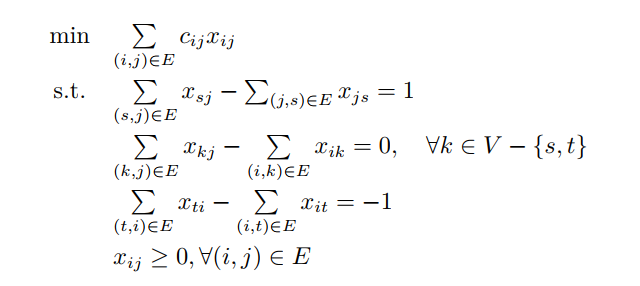
\includegraphics[width=0.8\textwidth]{图片1.png}
\end{figure}

\subsection{连通性}

LP算法中通过输出not\ found 报告该点与源点不连通。

dijksta算法通过比较最短路径的长度判断是否连通,若有边为正无穷则不连通。

\subsection{main函数}

\begin{figure}[H]
    \centering
    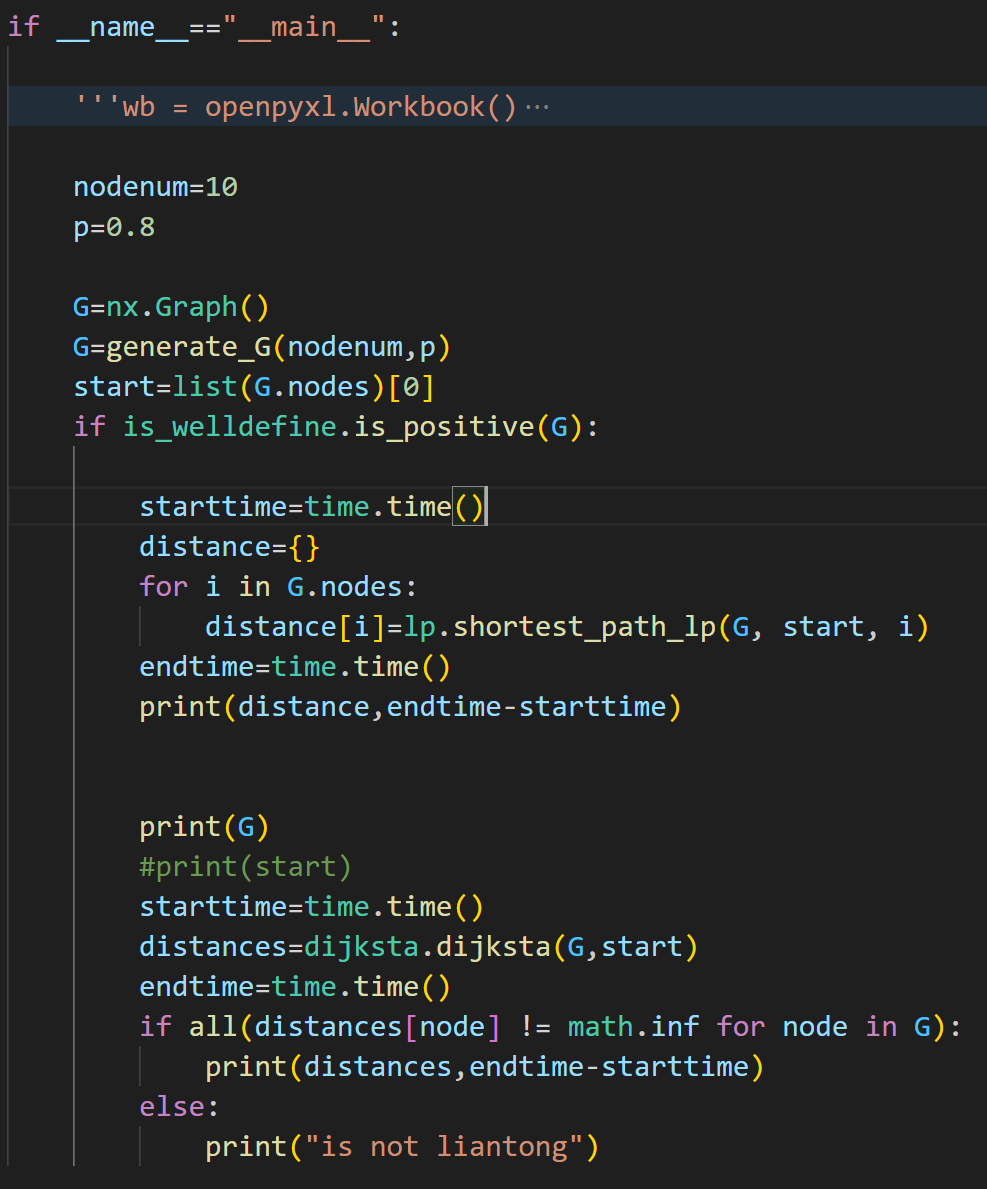
\includegraphics[width=0.5\textwidth]{屏幕截图 2024-10-18 133841.png}
\end{figure}

\begin{enumerate}
    \item 首先设置点数以及边生成概率
    \item 生成ER图
    \item 用LP方法对每个点求出其最短路径并记录时长
    \item 用dijksta方法求出最短路径并记录时长
    \item 注:因为当无法生成连通图时,有可能出现0点不存在情况,
    故我这里选$G$中第一个点为$start$。
\end{enumerate}

\section{实验结果}

\subsection{时间与节点数的关系}

\begin{figure}[H]
    \centering
    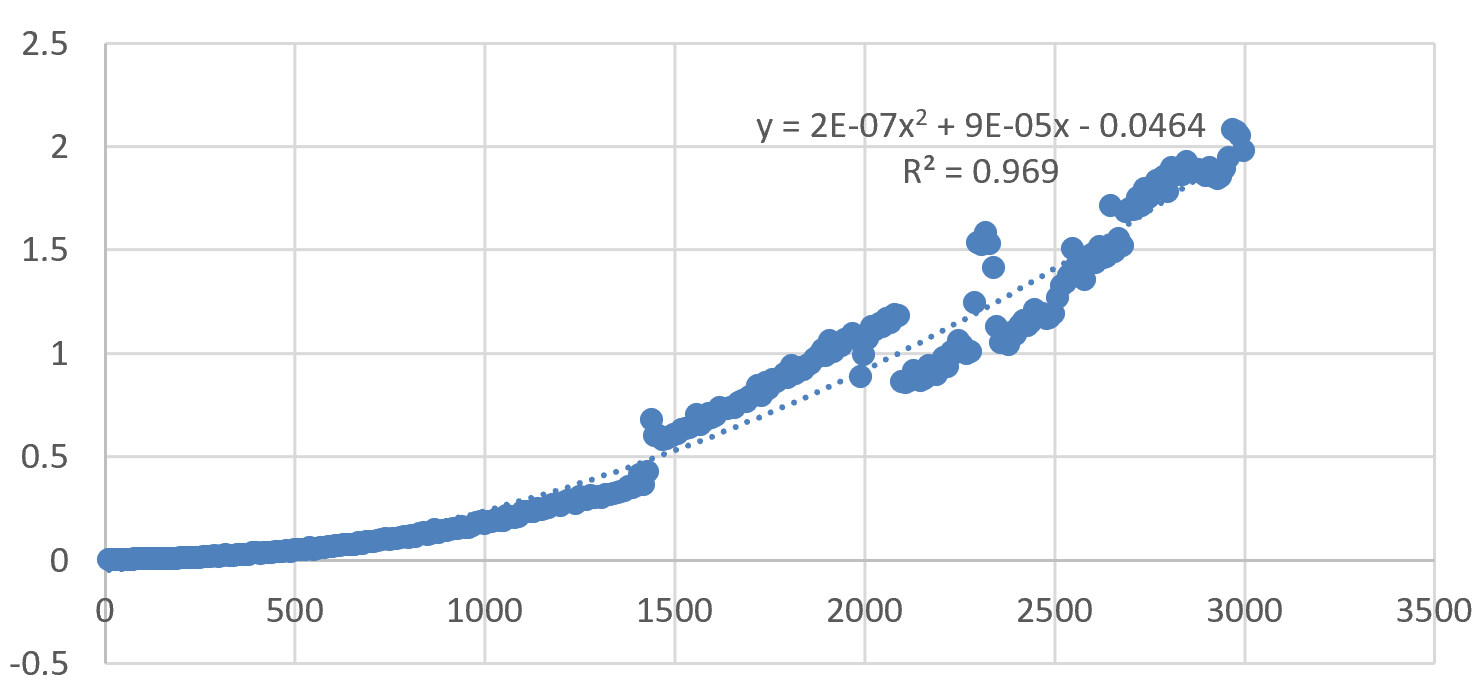
\includegraphics[width=0.8\textwidth]{屏幕截图 2024-11-05 100309.png}
    \caption{$time(s)-node$}
\end{figure}

\begin{figure}[H]
    \centering
    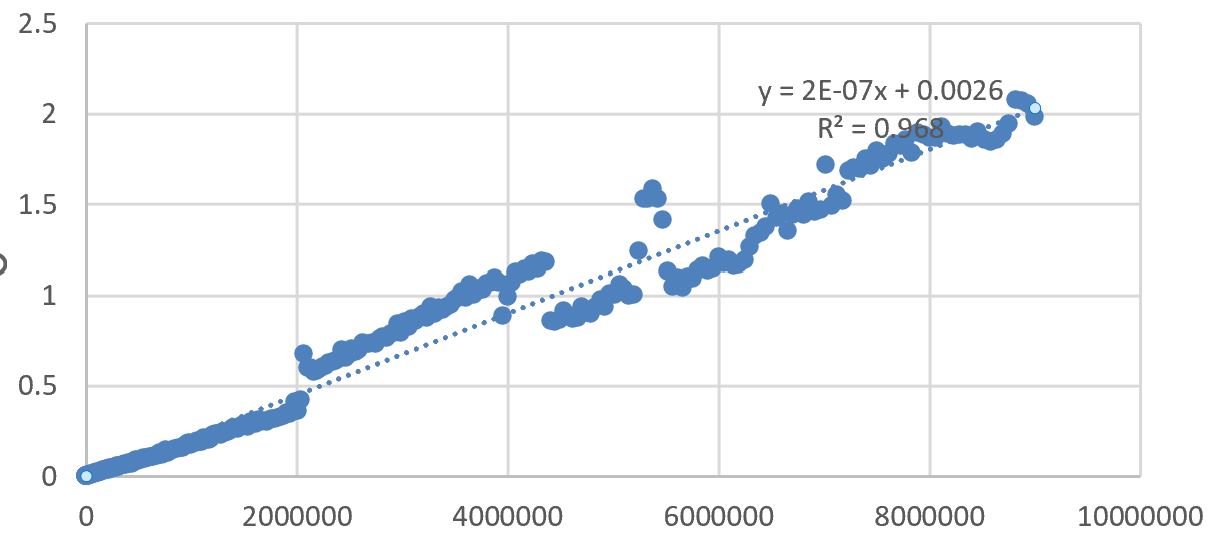
\includegraphics[width=0.8\textwidth]{屏幕截图 2024-11-05 100835.png}
    \caption{$time(s)-node^2$}
\end{figure}

我们对不同节点数的图进行实验,观察运行时间与节点数
之间的关系。实验中将节点数从10开始,以10为步长跑到
3000,每步运行10次并计算平均时间,得到如上结果:

做拟合可知运行时间和节点数大致成二阶线性,可能因为边数的不稳定会导致一些突变。

\subsection{与LP对比}
为了比较Dijkstra算法和LP方法的性能,我们统计了
在不同节点数下两种算法的运行时间。以下为部分实验
结果(以$n=10, 50, 100, 200, 500$为例):
\begin{table}[H]
    \centering
    \begin{tabular}{|c|c|c|}
        \hline
        n & LP & Dijksta\\
        \hline
        10 &0.07209038734436035 &0.0 \\
        \hline
        50 &0.8043262958526611 & 0.0\\
        \hline
        100 &4.852661848068237 &0.0 \\
        \hline
        200 &39.18767261505127&0.0\\
        \hline
        500& 1126.7072744369507&0.04920601844787598\\
        \hline
    \end{tabular}
\end{table}
可以看出,Dijkstra算法的效率明显优
于LP方法,尤其在节点数较小时,Dijks
tra算法几乎可以立即求解最短路径,而
LP方法则需要更多的计算时间。

\section{总结}

Dijksta优点:
\begin{enumerate}
    \item 高效性:在稠密图中,Dijkstra 算法能够快速求解最短路径。相比于其他如 Bellman-Ford 等算法,Dijkstra 不需要处理负权边,且在没有负权环的情况下,算法能够稳定地求解最短路径。
    \item 广泛应用:Dijkstra 算法被广泛应用于网络路由、地图导航等需要快速计算最短路径的场景。
\end{enumerate}

缺点:
\begin{enumerate}
    \item 性能瓶颈:当节点数和边数增加时,Dijkstra 算法的运行时间增长较快,尤其在大规模图中,可能导致计算效率不高。
    \item 不适用于负权边:Dijkstra 算法不能处理带有负权边的图,如果图中有负权边,则需要使用 Bellman-Ford 等算法。
\end{enumerate}



\end{document}
